\let\negmedspace\undefined
\let\negthickspace\undefined
\documentclass[journal]{IEEEtran}
\usepackage[a5paper, margin=10mm, onecolumn]{geometry}
\usepackage{lmodern} % Ensure lmodern is loaded for pdflatex
\usepackage{tfrupee} % Include tfrupee package

\setlength{\headheight}{1cm} % Set the height of the header box
\setlength{\headsep}{0mm}     % Set the distance between the header box and the top of the text

\usepackage{gvv-book}
\usepackage{gvv}
\usepackage{cite}
\usepackage{amsmath,amssymb,amsfonts,amsthm}
\usepackage{algorithmic}
\usepackage{graphicx}
\usepackage{textcomp}
\usepackage{xcolor}
\usepackage{txfonts}
\usepackage{listings}
\usepackage{enumitem}
\usepackage{mathtools}
\usepackage{gensymb}
\usepackage{comment}
\usepackage[breaklinks=true]{hyperref}
\usepackage{tkz-euclide} 
\usepackage{listings}
\usepackage{gvv}                                        
\def\inputGnumericTable{}                       
\usepackage[latin1]{inputenc}                                
\usepackage{color}                                            
\usepackage{array}                                            
\usepackage{longtable}                                       
\usepackage{calc}                                             
\usepackage{multirow}                                         
\usepackage{hhline}                                           
\usepackage{ifthen}                                           
\usepackage{lscape}  
\usetikzlibrary{patterns}
\begin{document}
\bibliographystyle{IEEEtran}
\textbf{Question 1.7.12:} \\
\textbf{} Find the value of $k$, if the points $P(5,4)$, $Q(7,k)$ and $R(9,-2)$ are collinear. 

\textit{Hint:} Three points $P(x_1,y_1)$, $Q(x_2,y_2)$, $R(x_3,y_3)$ are collinear if the area of the triangle formed by them is zero.\\
\\

\textbf{Solution}



\section*{Question}
Find the value of $a$, if the distance between the points 
$A\myvec{-3\\-14}$ and $B\myvec{a\\-5}$ is $9$ units.

\section*{Solution}
\begin{align}
\vec P=\myvec{5\\4},\qquad
\vec Q=\myvec{7\\k},\qquad
\vec R=\myvec{9\\-2}
\end{align}

 \textbf{Collinearity via rank}
Three points \(P,Q,R\) are collinear iff
\begin{align}
\operatorname{rank}\!\myvec{\; \vec Q-\vec P \;\; \vec R-\vec P \;}=1.
\end{align}
Compute the direction columns:
\begin{align}
\vec Q-\vec P=\myvec{7-5\\k-4}=\myvec{2\\k-4},\qquad
\vec R-\vec P=\myvec{9-5\\-2-4}=\myvec{4\\-6}.
\end{align}
Hence the collinearity matrix is
\begin{align}
M=\myvec{\,2 & 4\\ k-4 & -6\,}.
\end{align}

\textbf{Row reduction (rank\,=\,1)}
\begin{align}
\myvec{\,2 & 4\\ k-4 & -6\,}
\;\xrightarrow{\,R_1\leftarrow \tfrac12 R_1\,}\;
\myvec{\,1 & 2\\k-4 & -6\,}
\;\xrightarrow{\,R_2\leftarrow R_2-(k-4)R_1\,}\;
\myvec{\,1 & 2\\0 & 2(1-k)\,}.
\end{align}
For rank\((M)=1\), the second row must be the zero row:
\begin{align}
2(1-k)=0 \;\;\Rightarrow\;\; k=1.
\end{align}

\textbf{Conclusion}
For \(k=\boxed{1}\), the three points \(P(5,4),\,Q(7,k),\,R(9,-2)\) are collinear.

\newpage
\begin{figure}
    \centering
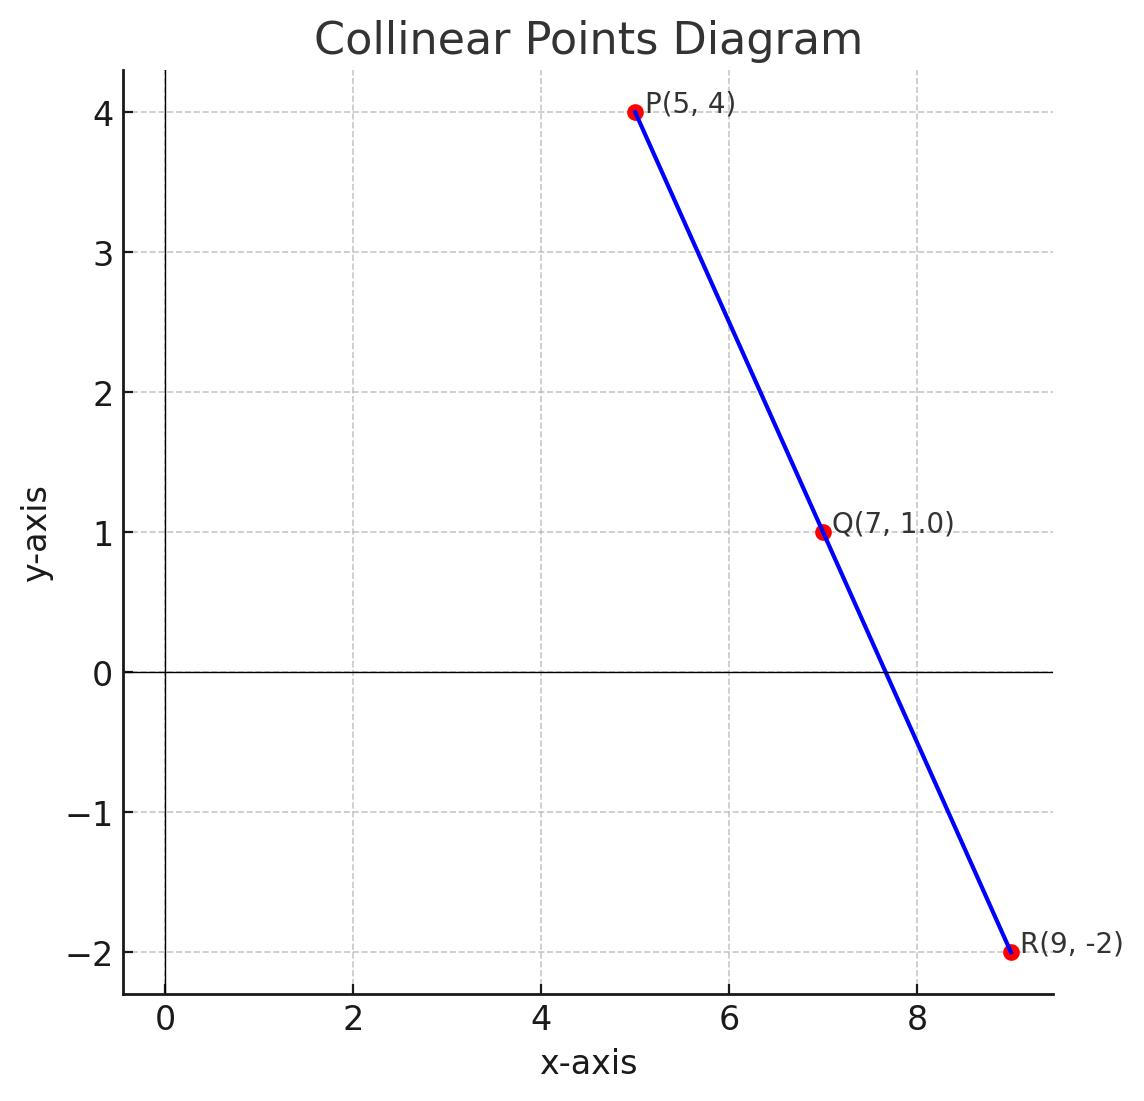
\includegraphics[width=0.5\linewidth]{figs/ASSIGN2.jpeg}
    \caption{}
    \label{fig:placeholder}
\end{figure}


\end{document}